\documentclass[12pt]{article}

\usepackage{amsmath}
\usepackage{amssymb}
\usepackage{graphicx}
\usepackage{tikz}

\counterwithin*{equation}{section}
\counterwithin*{equation}{subsection}

\graphicspath{ {./images/} } 

\begin{document}
\section{Equations of Lines} 

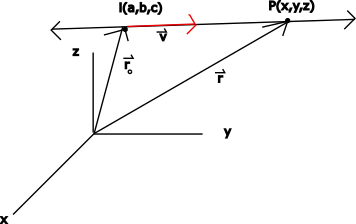
\includegraphics{line3d}
\fbox{$\vec{r} =\vec{r_0} +t \vec{v} $}

$t$ is the paramater of the equation.

Reiterate: $\vec{r} = \vec{r_0} +t \vec{IP} $

Let $\vec{v}=<a,b,c> $\\%
then $<x,y,z>=<x_0,y_0,z_0> + t<a,b,c>$\\%
$<x,y,z>=<x_0+ta,y_0+tb, z_0+tc>$

So the parametric equations for a line are as follows:
\begin{itemize}
	\item $x=x_0+ta$
	\item $y=y_0+tb$
	\item $z=z_0+tc$
\end{itemize}

When you solve for $t$, you get the \underline{symmetric equations}.\\%
$t=\frac{x-x_0}{a}=\frac{y-y_0}{b}=\frac{z-z_0}{c}$

If $b=0$, then you get:\\%
$\frac{x-x_0}{a}=\frac{z-z_0}{c}, y=y_0$

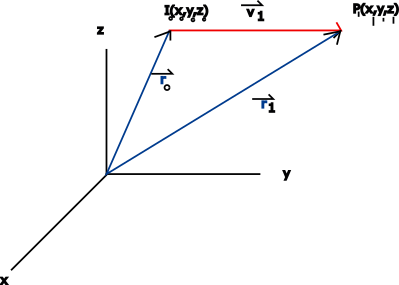
\includegraphics{3dline2}\\%
Lines in a 3D space can be parallel, intersecting, or skew.\\%
The figure above demonstrates $\vec{v_1}  $ which travels from $I(x,y,z)$ to $P(x,y,z)$\\%
Previously, we know $\vec{r} =\vec{r_0} +t \vec{v}    $\\%
Substitute $\vec{v} =\vec{r_1} -\vec{r_0}  $\\%
We get $\vec{r} =\vec{r_0} +t(\vec{r_1} -  \vec{r_0} )  $ \\%
$\vec{r} =  (1-t)\vec{r_0}  +t\vec{r_1}    $\\%
$0\leq t\leq1$, since the parameter $t$ limits the points to between I and P

\subsection{Equations of Lines Example 1}
Are the lines parallel, skew, or intersecting?\\%
$L_1: x = 2 + t,\ y = -1 + 3t,\ z = 5-t$\\%
$L_2: x = 1 + 2u,\ y = 4 + u,\ z = -2 + 4u$\\%
$\vec{v_1}=<1, 3, -1>  $\\%
$\vec{v_2} =<2,1,4> $\\%
Not scalar multiples, so they are not parallel.\\%
Solve for intersecting points:
\begin{align}
	x=2+t=1+2u\\%
	y=-1+3t=4+u\\%
	z=5-t=-2+4t
\end{align}
From (2) $\rightarrow$  \(t=\frac{u+5}{3}\)\\%
If the lines intersect, then the statements from (1) and (3) should be true when substituting t and u into the equations.
\\We can solve \(u\) first.
\begin{align}
	2+\frac{u+5}{3}=1+2u\\%
	2u-\frac{u+5}{3}=1\\%	
	\frac{5u-5}{3}=1\\%
	u = \frac{5}{8}
\end{align}
So \(t=\frac{\frac{5}{8}+5}{3}= \frac{45}{24}\)\\%
Now, we substitute the values and check for intersections.
\begin{align}
	x=2+\frac{45}{24}=1+2 (\frac{5}{8})\\%
	\frac{93}{24}=\frac{9}{4}
\end{align}
So we do not have an intersection\\%
Therefore the lines are skew.

\section{Equations of Planes}
A plane has an origin \(P_0(x_0,y_0,z_0)\) and normal vector \(\vec{n} \).\\%
The normal vector is a vector which is orthogonal to any line on the plane, and lines on the plane originate from the origin \(P_0(x_0,y_0,z_0)\) to an endpoint \(P(x,y,z)\). Thus, lines on the plane can be represented as \(\vec{P_0P} \). \\%
We can use two vectors, \(\vec{r}\) and  \( \vec{r_0} \) to point to the points \(P_0\) and \(P\) respectively. This is represented in the figure below.

We are working on
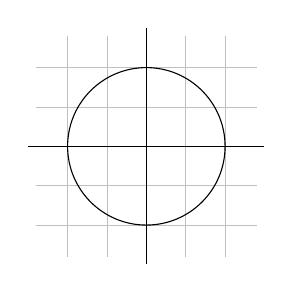
\begin{tikzpicture}
	\draw[step=0.5cm,lightgray,very thin] (-1.4,-1.4) grid (1.4,1.4);	
	\draw (-1.5,0) -- (1.5,0);
	\draw (0,-1.5,0) -- (0,1.5,0);
	\draw (0,0) circle (1cm);
\end{tikzpicture}.

\subsection{Incomplete do later}
Ex. 
Find where line L intersects plane $5x-2y+4z=18$

$L: x= -4t,\ y=5+t,\ z=2+3t$
\begin{align}
5(-4t)-2(5+t)+4(2+3t)=18\\
-20t-10-2t+8+12t=18\\
-10t=20\\
t=-2
\end{align}.
\begin{enumerate}
	\item Two planes are parallel if their normal vectors are parallel.
	\item Two planes that are not parallel intersect along a line
	\item The angle between intersecting planes is the angle between their normal vectors 
\end{enumerate}

Ex.: Consider planes $x+y+z=1$ and $3x+y-2z=1$
a) Find the angle between the planes
\subsection{Continued}
\begin{align}
	\vec{n_1}=<1,1,1>,\vec{n_2}=<3,1,-2> \\%
	\vec{n_1} \cdot {\vec{n_2}}=|\vec{n_1}||\vec{n_2}|\cos\theta 
\end{align}
Use the equations of two planes to describe a line\\%
Distance from a point to a plane\\%
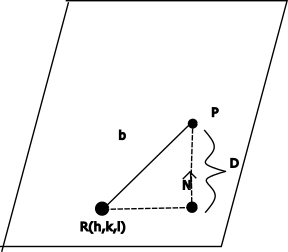
\includegraphics{ramppbn}\\%
$P_1(x_1,y_1,z_1)$\\%
$ax+by+cz+d=0$


EX: Find the distance between the parallel planes

\subsection
Ex: Find the distance between the lines $L_1$ and $L_2$ 

The distance between $L_1$ and $L_2$ is the same as the distance between the two parallel planes that contain these lines.\\
The normal vector $\vec{n}$ for these two planes must be orthogonal to $\vec{v_1}$ and $\vec{v_2}$
\end{document}


